\documentclass[tikz,border=2pt]{standalone}
\usepackage{amsmath}
\usepackage{pgfplots}
\pgfplotsset{compat=1.18}
\usetikzlibrary{arrows.meta}
\begin{document}
% Arrivals at 1,4,5,8,9,... (lambda = 1/2). Service time 1.5: D(t) stays within 2 of A(t), delta = 1/2 (rate-stable).
% Service time 2.5: D_k = 4 + 2.5(k-1), delta = 0.4 < lambda; at t = 40: A = 20, D = 19 and D = 15.
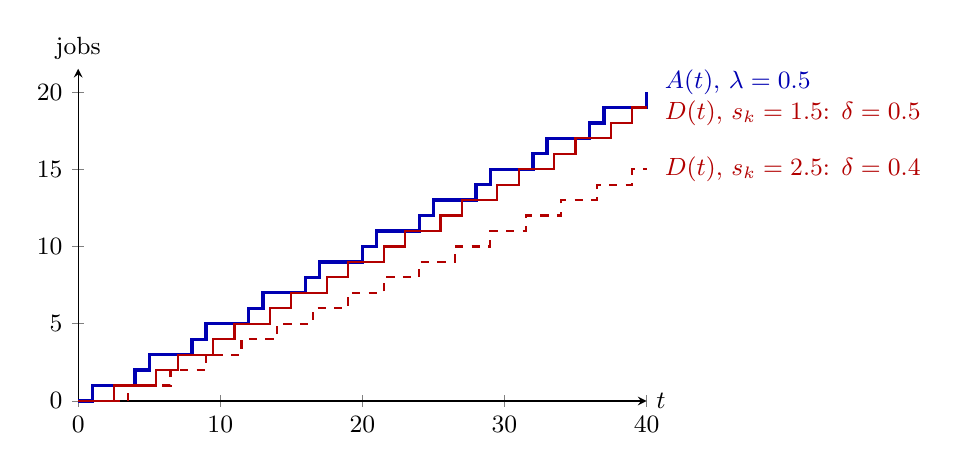
\begin{tikzpicture}[font=\small, >={Latex[length=2mm]}]
  \begin{axis}[
    axis lines=left, xmin=0, xmax=40, ymin=0, ymax=21.5,
    xtick={0,10,20,30,40}, ytick={0,5,10,15,20},
    xlabel={$t$}, ylabel={jobs},
    xlabel style={at={(axis description cs:1,0)}, anchor=west},
    ylabel style={rotate=-90, at={(axis description cs:0,1)}, anchor=south},
    width=8.8cm, height=5.8cm, clip=false
    ]
    \addplot[blue!70!black, very thick, const plot] coordinates {(0,0) (1,1) (4,2) (5,3) (8,4) (9,5) (12,6) (13,7) (16,8) (17,9) (20,10) (21,11) (24,12) (25,13) (28,14) (29,15) (32,16) (33,17) (36,18) (37,19) (40,20) (40,20)};
    \addplot[red!70!black, thick, const plot] coordinates {(0,0) (2.5,1) (5.5,2) (7,3) (9.5,4) (11,5) (13.5,6) (15,7) (17.5,8) (19,9) (21.5,10) (23,11) (25.5,12) (27,13) (29.5,14) (31,15) (33.5,16) (35,17) (37.5,18) (39,19) (40,19)};
    \addplot[red!70!black, thick, dashed, const plot] coordinates {(0,0) (3.5,1) (6.5,2) (9,3) (11.5,4) (14,5) (16.5,6) (19,7) (21.5,8) (24,9) (26.5,10) (29,11) (31.5,12) (34,13) (36.5,14) (39,15) (40,15)};
    \node[blue!70!black, anchor=west] at (axis cs:40.6,20.6) {$A(t)$, $\lambda=0.5$};
    \node[red!70!black, anchor=west] at (axis cs:40.6,18.6) {$D(t)$, $s_k=1.5$: $\delta=0.5$};
    \node[red!70!black, anchor=west] at (axis cs:40.6,15) {$D(t)$, $s_k=2.5$: $\delta=0.4$};
  \end{axis}
\end{tikzpicture}
\end{document}
